%% GuardLM paper — ACL style
\documentclass[11pt]{article}

\usepackage[preprint]{acl}
\usepackage{times}
\usepackage{latexsym}
\usepackage[T1]{fontenc}
\usepackage[utf8]{inputenc}
\usepackage{microtype}
\usepackage{inconsolata}
\usepackage{graphicx}
\usepackage{booktabs}
\usepackage{amsmath}
\usepackage{multirow}
\usepackage{xcolor}
\usepackage{tikz}
\usetikzlibrary{arrows.meta, positioning}

\title{GuardLM: A Single-GPU Alignment Pipeline for Structured\\Content-Safety Risk Detection in Chinese}

\author{Jianhua Guo \\
  Shenzhen University \\
  \texttt{1125448766@qq.com}}

\begin{document}
\maketitle

\begin{abstract}
Industrial content moderation still leans on keyword blocklists that are trivially evaded by homophone, pinyin, and character-splitting variants, while general-purpose LLMs do not reliably emit the structured verdicts that downstream moderation systems require. We present \textbf{GuardLM}, a 1.7B-parameter Chinese content-safety classifier built end-to-end on a single RTX~4090 (24\,GB). GuardLM couples (i) an adversarial data engine that unifies three public corpora at the 122k-text scale, fills scarce risk categories through scenario-matrix-constrained LLM synthesis, and manufactures 15.6k evasion variants; (ii) a three-stage alignment stack --- QLoRA SFT, DPO on preference pairs derived from error attribution, and GRPO with a four-component reward --- that raises overall F1 from 0.862 to 0.874 on a three-tier, leakage-checked benchmark; and (iii) a vLLM serving layer with JSON-schema-constrained decoding that pins the format error rate at 0.00\% with no measured throughput tax. Our analysis shows that DPO mostly \emph{migrates} errors between misses and false alarms rather than reducing them, whereas GRPO with an elevated sampling temperature (effective gradient groups 33\%$\rightarrow$50\%) breaks this trade-off and improves both ends simultaneously (adversarial recall +1.6\,pt, false-positive rate 3.57\%$\rightarrow$2.86\%). A deployment study quantifies serving trade-offs: AWQ 4-bit quantization costs 4.81-pt F1, concentrated in adversarial recall (homophone $-$18.2\,pt), so we retain bf16 serving, measured at 62.3\,req/s under concurrency 16 with P99 latency 266\,ms.
\end{abstract}

\section{Introduction}

Chinese online platforms moderate comments, danmaku, and private messages against several risk categories: pornography, insults, advertising diversion, and illegal content. Two deployment constraints shape the problem. First, \emph{lexical} defenses are brittle: a word blocklist can be evaded at near-zero cost by homophone substitution (\emph{xiéyīn}), pinyin initials, or character splitting (\emph{chāizì}), which real users employ routinely. Second, \emph{general-purpose} LLMs, although semantically capable, do not honor a fixed output contract: in our measurement, the untuned Qwen3-1.7B base model produced schema-compliant JSON for 0\% of inputs, emitting free-form risk commentary instead of the machine-parseable verdicts a rule engine consumes.

GuardLM closes this gap with a 1.7B specialized model that is deliberately small enough to train and serve on one consumer GPU. The full stack --- data engine, three-stage alignment, leakage-checked evaluation, and serving --- is designed, measured, and documented as a reproducible vertical-domain pipeline.

Our contributions are:
\begin{itemize}\itemsep1pt
\item \textbf{An adversarial data engine} that unifies COLD, Safety-Prompts, and CValues into a 122k-text pool, fills acutely scarce categories via a 20-cell scenario matrix that constrains LLM synthesis (porn 38$\rightarrow$156, ads 27$\rightarrow$201), and generates 15.6k evasion variants with five deterministic augmentation families, with MinHash deduplication and provenance tracking guaranteeing zero train--eval leakage.
\item \textbf{A three-stage alignment recipe} (QLoRA SFT $\rightarrow$ DPO $\rightarrow$ GRPO) on Qwen3-1.7B, with an \emph{evaluation-first} harness, error attribution that converts benchmark errors into preference pairs, and a temperature probe that revives GRPO group diversity after DPO sharpening.
\item \textbf{An error-migration analysis} showing DPO's net effect is internal error migration (miss $\leftrightarrow$ false alarm) with a flat total error count, while GRPO simultaneously improves adversarial recall and false-alarm rate --- breaking the trade-off that DPO could not.
\item \textbf{A deployment study} covering JSON-schema constrained decoding (format errors 0.2\%$\rightarrow$0.00\%, zero throughput tax), single-GPU capacity baselines (62.3\,req/s @ concurrency 16), and a quantization trade-off analysis leading to a data-driven rejection of AWQ 4-bit for the primary serving path.
\end{itemize}

\section{Related Work}

\paragraph{Chinese safety corpora and moderation.}
Public resources cover complementary slices of the safety problem: COLD \citep{yang2022cold} annotates offensive comments, Safety-Prompts \citep{safetyprompts} collects adversarial safety scenarios, and CValues \citep{cvalues2024} contributes safety-contrast question--answer pairs. None individually matches a production taxonomy of platform risks, and none covers graphonym-based evasion at scale; our data engine unifies them and manufactures the missing adversarial surface.

\paragraph{Alignment methods.}
RLHF with PPO \citep{schulman2017ppo} aligns models via a learned reward but is engineering-heavy. DPO \citep{rafailov2023dpo} reframes preference optimization as a closed-form classification loss, and GRPO \citep{shao2024deepseekmath} replaces the critic with group-relative advantages, enabling outcome-rewarded RL within the memory budget of a single GPU. We use both in sequence and analyze \emph{where each moves errors} rather than only aggregate scores.

\paragraph{Efficient fine-tuning and serving.}
LoRA \citep{hu2022lora} and QLoRA \citep{dettmers2023qlora} make full alignment stacks feasible on consumer GPUs; LLaMA-Factory \citep{zheng2024llamafactory} and TRL \citep{vonwerra2020trl} provide the training scaffolds. For serving, vLLM \citep{kwon2023vllm} introduced paged attention for high-throughput inference, XGrammar \citep{dong2024xgrammar} provides schema-constrained decoding, and AWQ \citep{lin2024awq} offers 4-bit activation-aware quantization. We measure the accuracy cost of quantization specifically for a small vertical-domain classifier, where, as we show, the damage concentrates in exactly the adversarial capabilities the model exists to provide.

\section{Task Formulation}

Given an input text $x$ (a comment, danmaku, or private message), the model must emit
\begin{equation}
y = \{\texttt{"label"}: \ell,\ \texttt{"risk"}: r,\ \texttt{"reason"}: s\},
\end{equation}
where $\ell \in \{$\texttt{porn}, \texttt{insult}, \texttt{ads}, \texttt{illegal}, \texttt{none}$\}$, $r \in [0,1]$ is a calibrated confidence, and $s$ is a one-line attribution. The contract is deliberately minimal: three fields are sufficient for a downstream rule engine to branch on, while the \texttt{reason} field keeps individual decisions auditable by human reviewers.

We treat the task as five-class classification with a per-tier false-positive discipline: in content safety, a \emph{miss} (risk text released) is operationally costlier than a \emph{false alarm} (benign text held), so we report recall on risk classes and the false-positive rate (FPR) on \texttt{none} alongside F1.

\section{Data Engine}

\subsection{Corpus unification}
We ingest three public sources: COLD (31{,}692 offensive-comment annotations), Safety-Prompts (89{,}997 adversarial scenarios across 10 risk families), and CValues (38{,}689 safe/unsafe answer pairs, used in M3 for preference construction). After schema unification to our five-label taxonomy, normalization, and filtering, the pool holds 122{,}183 texts; MinHash deduplication \citep{broder1997minhash} removes 33 fuzzy duplicates, leaving 122{,}150.

\subsection{Scenario-matrix synthesis}
The unified pool is severely imbalanced toward \texttt{insult} and \texttt{illegal}: before synthesis it contains only 38 \texttt{porn} and 27 \texttt{ads} training texts. Rather than scraping --- legally and operationally fraught --- we drive a commercial instruction-tuned LLM through a \textbf{20-cell scenario matrix}: $\{$category$\} \times \{$surface: comment / danmaku / private message / broadcast signal$\} \times \{$style: colloquial / formal / coded$\}$, with temperature-diverse prompting and a JSON-only response contract, in the spirit of Self-Instruct \citep{wang2023selfinstruct}. Each candidate is human-reviewed; 494 of 495 survived, raising \texttt{porn} to 156 (4.1$\times$) and \texttt{ads} to 201 (7.4$\times$).

\subsection{Adversarial augmentation}
A five-family deterministic rewriter manufactures the evasion surface that public datasets lack: homophone substitution, pinyin abbreviation, character splitting, emoji interleaving, and traditional-Chinese conversion. Each variant carries an \texttt{origin\_id} linking back to its seed. Augmentation yields 15{,}627 variants; training data mixes original and augmented texts at a 1:1 per-source ratio so that the model sees each attack pattern thousands of times while never losing the natural-text anchor.

\subsection{Leakage control and benchmark}
A naive pipeline risks evaluating on augmented neighbors of training texts. We enforce three controls: (i) MinHash near-duplicate removal across the full pool before split; (ii) split-first-then-augment ordering, so a variant never crosses the train/eval boundary; (iii) an automated leak check asserting zero intersection. The held-out benchmark is three-tier, 650 samples total: \textbf{T1} (250 conventional), \textbf{T2} (250 adversarial: six perturbation families, $n$ per family ranging 10--120), and \textbf{T3} (150 boundary cases: slang, coded, and euphemistic risks near the none boundary).

\begin{table}[t]
\centering\footnotesize
\setlength{\tabcolsep}{3pt}
\begin{tabular}{lrl}
\toprule
Component & Count & Note \\
\midrule
COLD texts & 31{,}692 & offensiveness \\
Safety-Prompts & 89{,}997 & 10 risk families \\
CValues pairs & 38{,}689 & preference source \\
\midrule
Unified pool & 122{,}183 & 5-label schema \\
After MinHash dedup & 122{,}150 & $-$33 near-dupes \\
Synthesized & 494 & reviewed; porn 4.1$\times$ \\
Adversarial variants & 15{,}627 & 5 families \\
\midrule
SFT instructions & 12{,}148 & risk:none 1:3 \\
DPO preference pairs & 2{,}176 & error attribution \\
GRPO prompt pool & 2{,}400 & attack-weighted \\
\midrule
Benchmark T1/T2/T3 & 250/250/150 & leakage-checked \\
\bottomrule
\end{tabular}
\caption{Data engine statistics.}
\label{tab:data}
\end{table}

\section{Alignment Pipeline}

\begin{figure*}[t]
\centering
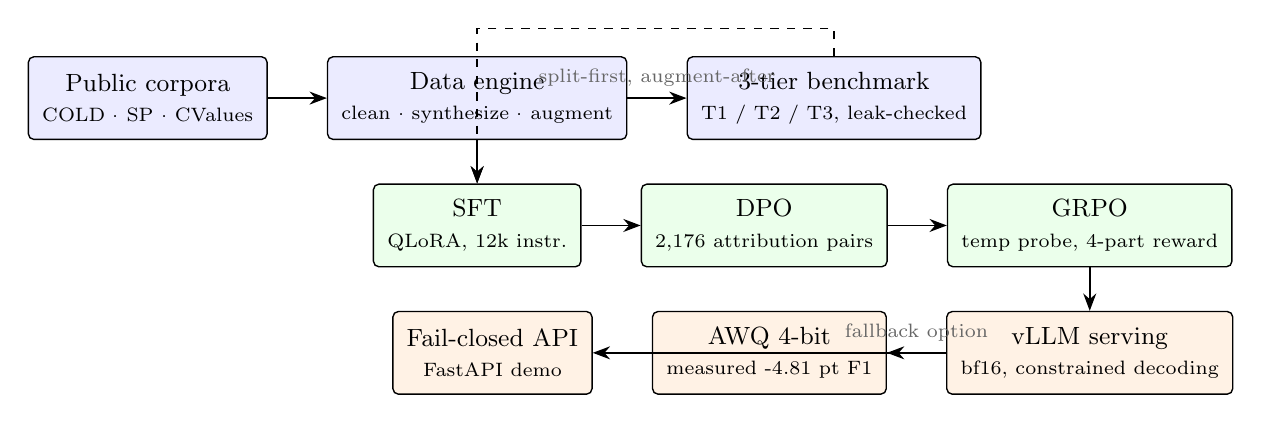
\begin{tikzpicture}[
  font=\small,
  node distance=0.55cm and 0.75cm,
  box/.style={draw, rounded corners=2pt, align=center, minimum height=1.05cm, inner sep=5pt, line width=0.5pt},
  data/.style={box, fill=blue!8},
  train/.style={box, fill=green!8},
  serve/.style={box, fill=orange!10},
  note/.style={font=\scriptsize, text=black!60, align=center},
  arr/.style={-{Stealth[length=2.2mm]}, line width=0.6pt}
]
\node[data] (corpora) {Public corpora\\ \scriptsize COLD · SP · CValues};
\node[data, right=of corpora] (engine) {Data engine\\ \scriptsize clean · synthesize · augment};
\node[data, right=of engine] (bench) {3-tier benchmark\\ \scriptsize T1 / T2 / T3, leak-checked};
\node[train, below=of engine] (sft) {SFT\\ \scriptsize QLoRA, 12k instr.};
\node[train, right=of sft] (dpo) {DPO\\ \scriptsize 2{,}176 attribution pairs};
\node[train, right=of dpo] (grpo) {GRPO\\ \scriptsize temp probe, 4-part reward};
\node[serve, below=of grpo] (vllm) {vLLM serving\\ \scriptsize bf16, constrained decoding};
\node[serve, left=of vllm] (awq) {AWQ 4-bit\\ \scriptsize measured -4.81 pt F1};
\node[serve, left=of awq] (demo) {Fail-closed API\\ \scriptsize FastAPI demo};
\draw[arr] (corpora) -- (engine);
\draw[arr] (engine) -- node[note, above=0.02cm] {split-first, augment-after} (bench);
\draw[arr] (engine) -- (sft);
\draw[arr] (sft) -- (dpo);
\draw[arr] (dpo) -- (grpo);
\draw[arr, dashed] (bench.north) -- ++(0,0.35) -| (sft.north);
\draw[arr] (grpo) -- (vllm);
\draw[arr] (vllm) -- (demo);
\draw[arr] (vllm) -- node[note, above=0.02cm] {fallback option} (awq);
\end{tikzpicture}
\caption{GuardLM pipeline. The benchmark feeds every stage through error attribution; the serving layer measures three deployment forms under one protocol.}
\label{fig:pipeline}
\end{figure*}

\subsection{Evaluation-first harness}
Before any training, we build a harness that runs batched inference, parses verdicts with a five-level JSON tolerance chain (strict parse $\rightarrow$ substring extraction $\rightarrow$ field-repair $\rightarrow$ heuristic label mapping $\rightarrow$ none-default), and emits per-tier Markdown reports. Running the untuned base model through it establishes the necessity baseline: 100\% format violations and unusable classification, motivating instruction tuning as stage one.

\subsection{Stage 1: SFT}
We fine-tune Qwen3-1.7B \citep{qwen3technical} with QLoRA \citep{dettmers2023qlora} on 12{,}148 instructions at a deliberate risk:none ratio of 1:3 --- the untuned base model exhibits a strong risk prior (86--96\% of texts judged risky), and negative reweighting is required to anchor the decision boundary. Training: rank 16, $\alpha$ 32, lr $10^{-4}$, effective batch 32, 3 epochs --- 1{,}083 steps in 12\,min 16\,s on one RTX 4090 (47.0 samples/s, 17.3\,GB peak VRAM), eval loss 0.0056 with no divergence. Result: format compliance 0\%$\rightarrow$99.8\%, overall F1 0.862, adversarial-tier (T2) recall 0.800.

\subsection{Stage 2: DPO from error attribution}
We bucket the 134 SFT errors into four causes: boundary misjudgment 42.5\%, adversarial failure 38.8\%, category confusion 17.9\%, format 0.7\%. Each error becomes a preference pair (chosen: the correct verdict with a faithful reason; rejected: the model's actual error), yielding 2{,}176 pairs. A first run at lr $5\times10^{-6}$ never left the $\ln 2$ loss floor; lr $10^{-5}$ learns but pushes FPR to a 3.57\% red line; adding 176 mirrored \texttt{none} pairs (chosen: none, rejected: over-blocked verdict) recovers the false-alarm direction while keeping boundary gains, adopted as dpo-v2 ($\beta=0.1$).

\subsection{Stage 3: GRPO with a temperature probe}
A GRPO \citep{shao2024deepseekmath} dry-run exposed a pathology inherited from DPO: the sharpened policy produced zero-advantage groups for 75--100\% of prompts (entropy 0.006), which starves the group-relative objective of gradient signal. A temperature probe over $\{1.0, 1.2, 1.5\}$ showed $T=1.5$ raises effective (non-degenerate) groups from 33\% to 50\% with zero format degradation --- diagnosis before tuning, not blind hyperparameter search. Final run: $T=1.5$, group size 8, $\beta_{\mathrm{KL}}=0.04$, lr $5\times10^{-6}$, one epoch over a 2{,}400 adversarial-weighted prompt pool, 300 steps in 24.8\,min.

\subsection{Reward design}
The reward has four components, each guarding one failure mode: \emph{correctness} (2.0, with incremental partial credit for near-miss categories) dominates; \emph{format} (1.0) locks the JSON contract; \emph{adversarial} boost ($\times$1.5) concentrates learning on evasion texts; and a \emph{length penalty} suppresses the classic RL output-inflation failure. Section~\ref{sec:dynamics} shows all four behaved as designed.

\section{Experiments}
\label{sec:exp}

\subsection{Setup}
All evaluation uses the 650-sample three-tier benchmark under a fixed protocol: temperature 0.7, top-$p$ 0.8, top-$k$ 20, max 64 new tokens, no chain-of-think mode; parse failures count as \texttt{none} (a held verdict), and the format error rate is reported separately. Iteration decisions are additionally protected by McNemar and Fisher exact tests on per-sample flips, with a pre-registered 2-pt red line beyond the $\pm$2\,pt noise band of a 650-sample benchmark.

\begin{table*}[t]
\centering\small
\begin{tabular}{llcccccc}
\toprule
Stage & Model & Overall F1 & T1 F1 & T2 F1 & T2 Recall & FPR & Format err. \\
\midrule
base & Qwen3-1.7B (untuned) & 0.000$^{*}$ & -- & -- & -- & -- & 100\% \\
SFT & sft-v1 & 0.8619 & 0.8731 & 0.8889 & 0.8000 & 0.71\% & 0.15\% \\
DPO & dpo-v2 & 0.8669 & 0.8500 & 0.8962 & 0.8120 & 3.57\% & 0.15\% \\
GRPO & grpo-v1 & \textbf{0.8740} & 0.8713 & \textbf{0.9059} & \textbf{0.8280} & \textbf{2.86\%} & \textbf{0.00\%} \\
\midrule
serving & guardlm-final (vLLM bf16) & 0.8755 & 0.8780 & 0.9011 & 0.8200 & 3.57\% & 0.00\% \\
serving & guardlm-awq (vLLM 4-bit) & 0.8274 & 0.8469 & 0.8558 & 0.7480 & 2.14\% & 0.00\% \\
\bottomrule
\end{tabular}
\caption{Main results on the 650-sample three-tier benchmark. $^{*}$The untuned base does not produce schema-compliant JSON (0\% compliance), so F1 is undefined; the row documents the necessity of instruction tuning. Serving rows reuse grpo-v1 weights under identical protocol.}
\label{tab:main}
\end{table*}

\subsection{Main results}
Table~\ref{tab:main} tracks the four training stages plus two serving forms. Overall F1 rises monotonically 0.000 $\rightarrow$ 0.862 $\rightarrow$ 0.867 $\rightarrow$ 0.874, and the vLLM bf16 deployment preserves it (0.8755, within the noise band, confirming zero serving loss). T3 (boundary) F1 improves 0.805 $\rightarrow$ 0.828 across SFT$\rightarrow$DPO, then holds within noise at GRPO (0.819; McNemar $p=0.688$ on the tier).

\subsection{DPO migrates errors; GRPO breaks the trade-off}
\label{sec:migration}
DPO's headline gain (T3 +2.3\,pt) hides its net effect: comparing per-sample outcomes across the benchmark, the \emph{total} error count is flat --- errors migrate between misses and false alarms rather than disappear, and FPR crosses the red line (0.71\%$\rightarrow$3.57\%). A KL check ($\mathrm{KL}(\pi\Vert\pi_{\mathrm{ref}})\approx0.001$ bits/token) rules out policy drift as the cause, pointing instead to the preference signal itself re-balancing along a single trade-off axis.

GRPO acts on the same benchmark with a different signature: 19 errors repaired vs.\ 10 regressed (net +9, McNemar $p=0.136$ overall; $p=0.092$ on T2, marginally significant) \emph{while simultaneously} lowering FPR 3.57\%$\rightarrow$2.86\% and raising adversarial recall 0.812$\rightarrow$0.828 --- both ends improve, which DPO could not achieve on this budget. Flip inspection shows the mechanism: repaired cases are adversarial \texttt{illegal}/\texttt{insult} misses, while the mirrored-\texttt{none} direction from the reward's partial credit restores over-blocked benign texts.

\subsection{Training dynamics}
\begin{figure*}[t]
\centering
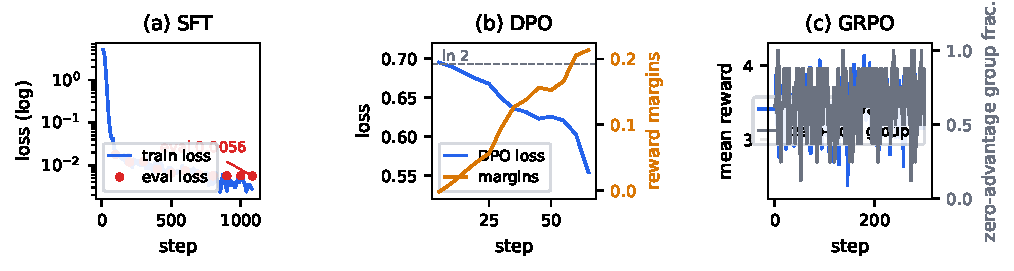
\includegraphics[width=\textwidth]{figures/alignment_curves.pdf}
\caption{Alignment-stage training curves from TensorBoard event logs. (a) SFT: train/eval loss, 1{,}083 steps in 12\,min; eval loss bottoms at 0.0056 with no overfitting fork. (b) DPO: loss escapes the $\ln 2$ floor as reward margins separate. (c) GRPO: mean reward rises 2.39$\rightarrow$4.13 while zero-advantage group fraction collapses 1.0$\rightarrow$0.125 after the temperature probe.}
\label{fig:curves}
\end{figure*}

\begin{figure*}[t]
\centering
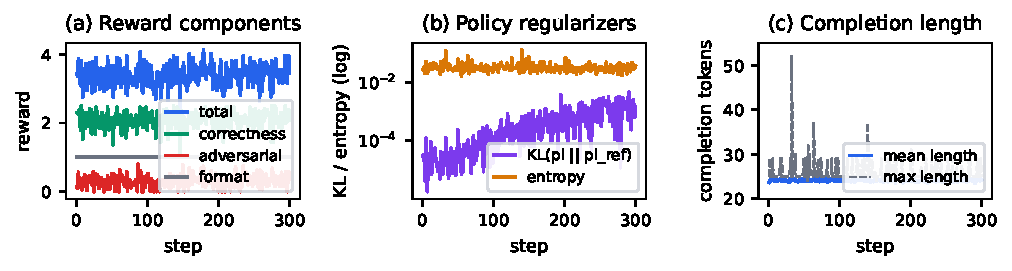
\includegraphics[width=\textwidth]{figures/grpo_health.pdf}
\caption{GRPO training health over 300 steps. (a) Reward components: correctness dominates and rises; the adversarial bonus activates on evasion prompts; format stays saturated. (b) KL to the reference stays below $5\times10^{-3}$ and entropy remains in 0.017--0.134 (log scale) --- mild policy movement, no collapse. (c) Completion length holds at 23--25 tokens (max 52): zero RL length drift, validating the length-penalty component.}
\label{fig:health}
\end{figure*}

Figure~\ref{fig:curves} shows the three training stages from event-log scalars. SFT converges smoothly; DPO's loss separates from $\ln 2$ only at the corrected learning rate, with margins growing to 0.214; GRPO's reward climbs while the zero-advantage fraction falls to 0.125 --- direct evidence that the temperature probe fixed the group-diversity pathology. Figure~\ref{fig:health} shows the run stayed healthy end-to-end: KL bounded, entropy away from zero, completions short and stable.

\subsection{Ablation: continued pre-training}
\label{sec:cpt}
A controlled ablation adds domain continued pre-training (CPT, 109k documents, 70\% risk text) before the identical SFT recipe (sft-v2). Domain slang generalization improves sharply: the P5 argot probe F1 0.824$\rightarrow$0.947 (+12.4\,pt), overall F1 0.898, adversarial recall 0.868. But the risk-heavy corpus re-introduces the risk prior on the pre-training side: FPR rises 0.71\%$\rightarrow$9.29\% --- the miss/false-alarm trade-off resurfaces at a deeper layer. Catastrophic-forgetting probes (chitchat, commonsense, arithmetic) all pass, and the experiment achieves its ablation purpose, but production keeps grpo-v1; replay-mixed CPT remains the open compromise.

\subsection{Ablation: 4-bit quantization}
\label{sec:awq}

\begin{table}[t]
\centering\small
\setlength{\tabcolsep}{4pt}
\begin{tabular}{lccc}
\toprule
Deployment & F1 & Recall & Weight \\
\midrule
HF transformers (bf16) & 0.8740 & 0.7824 & 3.3\,GiB \\
vLLM (bf16) & 0.8755 & 0.7863 & 3.3\,GiB \\
vLLM (AWQ 4-bit) & 0.8274 & 0.7098 & 1.3\,GiB \\
\bottomrule
\end{tabular}
\caption{Three deployment forms of grpo-v1 weights, identical 650-sample protocol. AWQ trades 4.81-pt F1 (Recall $-$7.65\,pt) for 61\% smaller weights and 2.6$\times$ faster batch inference (183\,s$\rightarrow$69\,s).}
\label{tab:quant}
\end{table}

\begin{table}[t]
\centering\small
\setlength{\tabcolsep}{5pt}
\begin{tabular}{lrrr}
\toprule
Perturbation & $n$ & bf16 R & AWQ R \\
\midrule
homophone & 22 & 90.9 & 72.7 \\
split & 10 & 90.0 & 80.0 \\
sp\_attack & 120 & 73.3 & 64.2 \\
emoji & 25 & 96.0 & 92.0 \\
pinyin & 26 & 76.9 & 73.1 \\
traditional & 47 & 93.6 & 93.6 \\
\bottomrule
\end{tabular}
\caption{T2 adversarial recall by perturbation type, bf16 vs.\ AWQ (\%). Character-level evasions collapse under 4-bit noise; semantic-level evasions survive.}
\label{tab:perturb}
\end{table}

Table~\ref{tab:quant} compares three deployment forms under one protocol. vLLM bf16 costs nothing (F1 $+$0.15\,pt, within noise). AWQ 4-bit costs 4.81\,pt F1, and Table~\ref{tab:perturb} localizes the damage: character-level evasions (homophone $-$18.2\,pt, split $-$10.0\,pt, sp\_attack $-$9.1\,pt) collapse while semantic-level perturbations (traditional, emoji) are nearly unaffected. Confusion-matrix deltas confirm the mechanism: false negatives rise 109$\rightarrow$148 while false positives fall --- quantization flattens boundary logits and shifts the whole decision mass toward \texttt{none}. For a 1.7B model whose weight redundancy is already thin, AWQ's 1\% salient-weight protection does not cover the discriminative region this task lives in. Because a miss is costlier than a false alarm in content safety, we reject AWQ for the primary path and keep it as a measured fallback for $\le$8\,GB-VRAM or offline pre-screening deployments.

\section{Deployment}

\paragraph{Constrained decoding.}
The serving layer turns format assurance from a post-hoc check into a decoding-time guarantee: vLLM's \texttt{json\_schema} guided decoding (XGrammar backend) masks logits against the output contract throughout generation. Measured effect: format errors 0.2\%$\rightarrow$0.00\% under the serving protocol, at zero throughput tax --- structured decoding on/off leaves request rate unchanged and costs $-$0.17\,pt F1, inside the noise band. The five-level parse fallback in the demo layer remains as defense in depth.

\begin{table}[t]
\centering\small
\begin{tabular}{crrr}
\toprule
Concurrency & req/s & P99 E2E & TTFT P99 \\
\midrule
1 & 28.2 & 35\,ms & 27\,ms \\
4 & 49.5 & 81\,ms & 45\,ms \\
16 & 62.3 & 266\,ms & 74\,ms \\
\bottomrule
\end{tabular}
\caption{Single-GPU serving capacity (bf16, constrained decoding on, stable in-flight load).}
\label{tab:capacity}
\end{table}

\paragraph{Capacity.}
Table~\ref{tab:capacity} reports the steady-state capacity baseline on one RTX 4090 with prefix caching disabled (kept off so the numbers are reproducible): 62.3\,req/s at concurrency 16 with P99 end-to-end latency 266\,ms --- comfortably within interactive moderation budgets.

\paragraph{Fail-closed discipline.}
The FastAPI gateway follows a fail-closed contract: if the inference backend is unreachable or a verdict cannot be parsed, it returns an explicit 502 rather than a fabricated verdict. In content safety, silently defaulting to \texttt{none} on backend failure would widen the miss rate exactly when the system is degraded; an explicit refusal routes the text to a fallback queue instead.

\section{Conclusion}

GuardLM demonstrates that a complete vertical-domain risk-identification stack --- adversarial data engine, three-stage alignment, leakage-checked three-tier evaluation, and quantitatively characterized serving --- fits on a single consumer GPU while reaching 0.874 overall F1 and 0.00\% format errors in production form. Two findings travel beyond this domain: (i) DPO applied to a classifier trades misses against false alarms without shrinking total error, while GRPO at a probed sampling temperature improves both ends at once; and (ii) post-training quantization of a small specialized classifier silently destroys exactly the adversarial capabilities it was built for, so the bf16/quantized decision must be measured, not assumed. The data engine, harness, training recipes, and deployment trade-offs are documented for reproduction.

\section*{Limitations}

The benchmark is 650 samples; improvements within $\pm$2\,pt are inside the noise band, and we used significance tests rather than raw deltas for all iteration decisions, but a larger tier-3 set would sharpen boundary conclusions. All results use one base model (Qwen3-1.7B) and Chinese only; cross-lingual transfer of the augmentation families is untested. Synthesis relied on a commercial LLM API whose exact model changed over the project's lifetime; the 494 surviving samples are human-reviewed, but the approach inherits any upstream alignment biases. CPT ablation suggests replay-mixed continued pre-training could resolve its FPR regression, but this remains future work, as do quantization-aware fine-tuning alternatives (GPTQ-INT8, QAT) that might close the 4.81-pt AWQ gap.

\bibliography{refs}

\end{document}
